\documentclass[10pt]{article}
\usepackage[a4paper,margin=1.78cm]{geometry}
\usepackage[T1]{fontenc}
\usepackage{lmodern,microtype}
\usepackage{amsmath,amssymb,amsthm,mathtools}
\usepackage{booktabs,array,enumitem,float}
\usepackage{graphicx,xcolor}
\usepackage[hidelinks]{hyperref}
\usepackage[nameinlink]{cleveref}
\setlist{nosep,leftmargin=*}
\newtheorem{theorem}{Theorem}[section]
\newtheorem{proposition}[theorem]{Proposition}
\newtheorem{lemma}[theorem]{Lemma}
\newtheorem{corollary}[theorem]{Corollary}
\newtheorem{remark}[theorem]{Remark}
\newcommand{\R}{\mathbb R}
\newcommand{\C}{\mathbb C}
\newcommand{\mcD}{\mathcal D}
\newcommand{\ip}[2]{\langle #1,#2\rangle}
\newcommand{\dd}{\,\mathrm d}
\newcommand{\Tr}{\operatorname{Tr}}
\newcommand{\spec}{\operatorname{spec}}
\newcommand{\Id}{\mathrm I}
\hypersetup{pdftitle={Certified Localized Weil Positivity Through Support 0.72},pdfauthor={Lluis Eriksson}}

\title{\bfseries Certified Localized Weil Positivity Through Support $0.72$:\\
Multiband Schur Complements and a Complete Stieltjes Hierarchy}
\author{Lluis Eriksson\\Independent Researcher\\\texttt{lluiseriksson@gmail.com}}
\date{August 2026}

\begin{document}
\maketitle

\begin{abstract}
Suzuki's localized Weil form is represented by a lower-bounded self-adjoint
operator $A_a$ on $L^2(-a,a)$; nonnegativity for every $a>0$ is equivalent to the
Riemann hypothesis, while positivity at one fixed support is an unconditional
and strictly weaker problem.  We give a source-level interval certificate for
the fixed-support inequality
\[
 A_{0.72}\succeq 5.890\times10^{-17}\Id>0.
\]
Nested-core monotonicity then gives the same scalar lower bound for every
$0<a\le0.72$.  The proof is not a positive Ritz computation.  It decomposes
the exact prime-power translation graph through $n=4$ into thirteen intervals, retains
endpoint and singular directions as interval Gram matrices, and bounds the
infinite complement by a mode-sensitive Schur estimate.  The decisive split
isolates degrees $12,\ldots,23$, followed by $[24,176)$ and $[176,\infty)$;
both parity Schur matrices have
78 certified positive directions and no unresolved direction at 512-bit Arb
precision.
An independent shadow implementation, importing neither the project nor
python-flint, reconstructs the prime-power graph and parity maps and
reassembles the exported Schur balls with high-precision arithmetic; it is a
wiring audit rather than a substitute for the Arb proof.

Two analytic results explain why this certificate scales beyond a single
matrix.  First, the boundary potential
$-\tfrac12\log(1-x^2)$ has an exact Gauss--Stieltjes hierarchy whose finite
approximants increase by explicit Schur squares and whose Markov remainder is
a continuous square.  At every fixed support this is a complete terminating
strict-positivity hierarchy.  Second, harmonic complement denominators admit
a $(1+\varepsilon)$ Loewner Schur majorant with only
$O_\varepsilon(\log\log M)$ bands through degree $M$.  The ingredients of
Gaussian quadrature and operator antitonicity are classical; the contribution
is their source-faithful integration with the arithmetic translations into a
rigorous coercivity certificate.  This is a bounded-support theorem, not a
proof of the Riemann hypothesis.
\end{abstract}

\noindent\textbf{Keywords.} Weil quadratic form; Riemann zeta function;
localized operator; interval arithmetic; Schur complement; Gauss quadrature;
Stieltjes function; Legendre expansion.

\section{Statement, context, and claim boundary}

Let $Q_W$ denote the global Weil quadratic form in Suzuki's additive
logarithmic convention, and let $Q_W^a$ be its closed restriction to functions
supported in $(-a,a)$.  Suzuki constructs the representing self-adjoint
operator $A_a$ on $L^2(-a,a)$ and identifies
\begin{equation}\label{eq:lambda-def}
 \lambda_a:=\min\spec(A_a)=
 \inf_{0\ne v\in C_c^\infty(-a,a)}
 \frac{Q_W(v)}{\|v\|_2^2}.
\end{equation}
The form is continuous in $a$, positive for sufficiently small support, and
the global Weil criterion asks for nonnegativity at every support
\cite{Suzuki2026,Yoshida1992,Bombieri2000}.  A finite-support lower bound is
therefore meaningful but cannot by itself decide the Riemann hypothesis.

Our main result is the following computer-assisted theorem.  All finite
quantities in its proof are outward-rounded real balls; floating eigenvectors
are used only to propose a congruence and never to decide a sign.

\begin{theorem}[localized coercivity]\label{thm:main}
In Suzuki's normalization of the global localized Weil form,
\begin{equation}\label{eq:main}
 \boxed{A_{0.72}\succeq
 5.890\times10^{-17}\Id>0.}
\end{equation}
Consequently, for every $0<a\le0.72$,
\begin{equation}\label{eq:interval}
 \lambda_a\ge5.890\times10^{-17}.
\end{equation}
\end{theorem}

The endpoint $0.72$ is not claimed optimal.  Among the primary sources we
located, the previous explicit rigorous localized radius is Yoshida's
$a=(\log2)/2$ result, reproduced and discussed by Bombieri
\cite{Yoshida1992,Bombieri2000}.  Connes--Consani report larger numerical
tests, and Kim et al. give a finite-element realization of Suzuki's operator,
but positive Ritz values are upper bounds and do not certify coercivity
\cite{ConnesConsani2023,KimEtAl2026}.  The present endpoint crosses the active
prime-power channels $n=2,3,4$, since $4<e^{1.44}<5$.

\begin{remark}[not the semilocal scaling Hamiltonian]
The operator in \cref{thm:main} is only the self-adjoint representative of
Suzuki's closed global localized form.  We do not identify it with a semilocal
Connes--Consani operator: that formulation has a different sign convention,
two moment constraints, multiplicative convolution, and a globally normalized
principal value.  No operator ordering between different $a$ is asserted,
because the operators act on different Hilbert spaces.
\end{remark}

\section{Source normalization and nested-core monotonicity}

We record the normalization because a wrong polar Gram changes the odd sector.
Put
\[
 \widehat v(z)=\int_\R v(x)e^{izx}\dd x,
 \qquad \widetilde v(x)=\overline{v(-x)},
 \qquad f=v*\widetilde v.
\]
Then $f(0)=\|v\|_2^2$.  In the direct explicit-formula representation the
polar contribution is
\begin{equation}\label{eq:polar}
 V_+\overline{V_-}+V_-\overline{V_+}
 =2\operatorname{Re}(V_+\overline{V_-}),
 \qquad V_\pm=\int v(x)e^{\pm x/2}\dd x,
\end{equation}
not $|V_+|^2+|V_-|^2$.  The scalar term is
$-(\log(4\pi)+\gamma)\|v\|_2^2$, while the arithmetic part is
\begin{equation}\label{eq:prime}
 -\sum_{n\ge2}\frac{\Lambda(n)}{\sqrt n}
   \bigl[f(\log n)+f(-\log n)\bigr].
\end{equation}
For support $[-a,a]$ the unsampled archimedean tail contributes the exact
$-2\operatorname{atanh}(e^{-2a})f(0)$ inside the archimedean integral.  These
conventions agree with Suzuki's global form and are independently exercised by
the source code.

\begin{proposition}[nested-core monotonicity]\label{prop:monotone}
If $0<a'\le a$, then $\lambda_{a'}\ge\lambda_a$.  In particular,
$A_a\succeq c\Id$ implies $\lambda_{a'}\ge c$ for all $a'\le a$.
\end{proposition}
\begin{proof}
Extension by zero embeds $C_c^\infty(-a',a')$ into
$C_c^\infty(-a,a)$ and preserves both the $L^2$ norm and the value of the
same global functional $Q_W$.  The admissible Rayleigh quotients for the
smaller interval are therefore a subset of those for the larger interval.
Apply \eqref{eq:lambda-def}.  This compares scalar infima, not operators on
different spaces.
\end{proof}

Thus the numerical-analytic burden is entirely at the largest endpoint.
Continuity additionally implies that, if the Riemann hypothesis is false, the
negative set of $\lambda_a$ is an upper open interval.  A zero plateau is not
excluded, so no simple or transverse crossing is claimed.

\section{The scale-free dominant operator}

After scaling $(-a,a)$ to $(-1,1)$, the dominant archimedean form is
\begin{equation}\label{eq:L}
 \mathcal L=A_2+V,\qquad
 (A_2w)(x)=\frac12\int_{-1}^1
 \frac{w(x)-w(y)}{|x-y|}\dd y,\qquad
 V(x)=-\frac12\log(1-x^2).
\end{equation}
The regional logarithmic Laplacian is exactly diagonal in the Legendre basis:
\begin{equation}\label{eq:harmonic}
 A_2P_n=H_nP_n,\qquad H_n=\sum_{k=1}^n\frac1k,\quad H_0=0,
\end{equation}
as established in the recent analysis of the interval logarithmic Laplacian
\cite{RosenzweigStanfill2026}.  The remaining bounded block contains the
scalar, smooth, and finitely many translation terms.  For $a=0.72$ its active
arithmetic displacements are $\log2/a$, $\log3/a$, and $\log4/a$; the last
weight is $-\Lambda(4)/2=-\log2/2$, not $-\log4/2$.

Cutting the interval at all translation endpoints gives thirteen subintervals.
Their pointwise translation graph has components of sizes seven, four, and
two.  Local normalized Legendre coordinates turn every exact translation
between equal-length intervals into an identity block.  The finite source
keeps twelve local degrees on each interval.  Reflection reduces the resulting
156-dimensional source into two $78\times78$ parity blocks.

\begin{proposition}[exact third-window partition]\label{prop:partition}
Suppose
\[
 \log2<a<\frac12\log\frac92,
 \qquad h_2=\frac{\log2}{a},\qquad h_3=\frac{\log3}{a}.
\]
In the scaled interval $[-1,1]$, the ordered cut points are
\begin{align*}
 -1,&\ 1-2h_2,\ -1+2h_2-h_3,\ 1-h_3,\ -1-h_2+h_3,\\
 &1-3h_2+h_3,\ -1+h_2,\ 1-h_2,\ -1+3h_2-h_3,\\
 &1+h_2-h_3,\ -1+h_3,\ 1-2h_2+h_3,\ -1+2h_2,\ 1.
\end{align*}
Numbering the resulting intervals $0,\ldots,12$, translations by $h_2$,
$h_3$, and $2h_2$ pair respectively
\begin{align*}
 &(0,6),(1,7),(2,8),(3,9),(4,10),(5,11),(6,12),\\
 &(0,10),(1,11),(2,12),\qquad (0,12).
\end{align*}
Hence the translation graph components are
\[
 \{0,2,4,6,8,10,12\},\qquad
 \{1,5,7,11\},\qquad \{3,9\}.
\]
All intervals in one component have the same length.
\end{proposition}
\begin{proof}
The endpoints are the orbit of $\{-1,1\}$ required to make the three
translations map whole cells to whole cells.  Their consecutive differences
repeat the three values
\[
 2(1-h_2),\qquad 4h_2-h_3-2,
 \qquad 2h_3-h_2-2.
\]
The first is positive because $a>\log2$; the third is positive exactly when
$2a<\log(9/2)$; and the middle is then positive as well because
$\log(9/2)<\log(16/3)$.  This proves the ordering.  Direct subtraction of
paired endpoints gives the three edge lists.  Graph connectivity gives the
components; their interval lengths are respectively the first, second, and
third displayed values.  For $a=0.72$, the window inequalities hold.
\end{proof}

Thus the arithmetic term in the local orthonormal Legendre basis is an exact
weighted graph matrix: every listed $n$-edge is
$-\Lambda(n)/\sqrt n$ times an identity block.  In particular, the sole
$n=4$ edge has coefficient $-\log2/2$.  This algebraic partition, rather than
a sampled quadrature grid, is what the interval source generator encloses.

\begin{figure}[H]
 \centering
 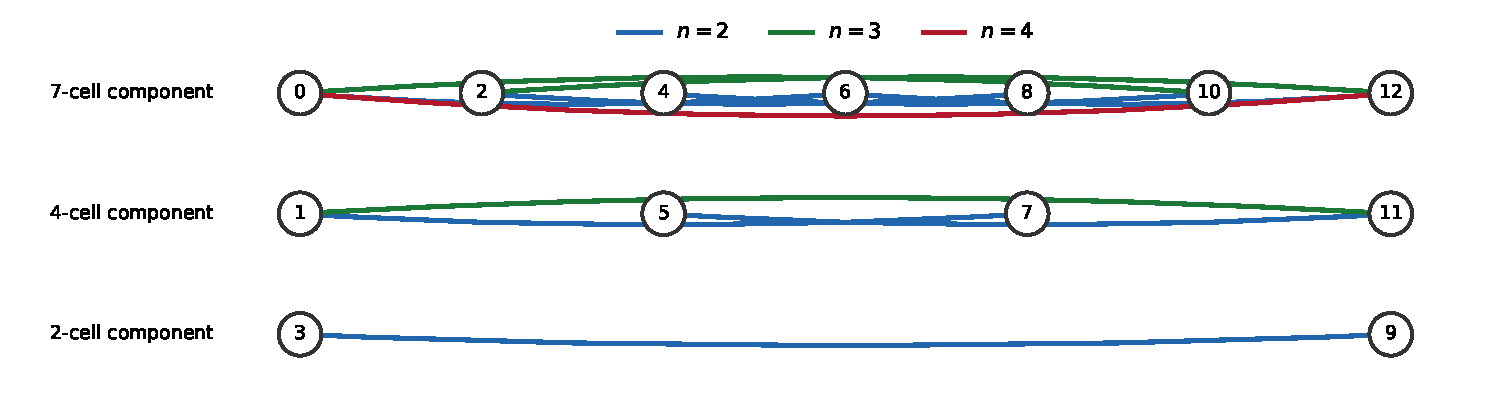
\includegraphics[width=0.93\linewidth]{figures/prime_translation_graph.pdf}
 \caption{Exact translation graph of the thirteen interval cells.  Each row
 is one pointwise connected component; edge colors record the prime-power
 channel.  The layout is schematic, while the vertex labels and edge set are
 the exact data used by the source generator.}
 \label{fig:translation-graph}
\end{figure}

\section{An exact Gauss--Stieltjes hierarchy}

The positive boundary potential can be retained rather than paid as a norm.
Set $y=x^2$.  The elementary Stieltjes identity
\begin{equation}\label{eq:stieltjes}
 V(x)=\frac12\int_0^1\frac{y}{1-ty}\dd t
\end{equation}
leads to a hierarchy that we now make explicit.  Let $(t_j,w_j)_{j=1}^m$ be
the $m$-node Gauss--Legendre rule on $[0,1]$ and define
\begin{equation}\label{eq:Rm}
 R_m(x)=\frac12\sum_{j=1}^mw_j\frac{x^2}{1-t_jx^2}.
\end{equation}

\begin{theorem}[exact Stieltjes hierarchy]\label{thm:stieltjes}
For $0<|x|<1$,
\begin{align}
 0<R_1(x)<R_2(x)<\cdots<V(x),\label{eq:nested}\\
 R_m(1)=H_m,\label{eq:endpoint}
\end{align}
where the endpoint value means the finite rational limit.  If
$p_m(t)=P_m(2t-1)$ and $q_m(y)=y^mp_m(1/y)$, then
\begin{equation}\label{eq:markov-square}
 V(x)-R_m(x)=\frac12\int_0^1
 \left(\frac{x^{2m+1}p_m(t)}
 {q_m(x^2)\sqrt{1-tx^2}}\right)^2\dd t.
\end{equation}
Let $J_m$ be the shifted-Legendre Jacobi matrix, with diagonal $1/2$ and
links
\[
 a_k=\frac{k}{2\sqrt{(2k-1)(2k+1)}}.
\]
Then
\begin{equation}\label{eq:resolvent}
 R_m(x)=\frac{x^2}{2}e_0^T(\Id-x^2J_m)^{-1}e_0,
\end{equation}
and, writing $A_m=\Id-x^2J_m$ and
\[
 s_m=1-\frac{x^2}{2}-x^4a_m^2e_{m-1}^TA_m^{-1}e_{m-1}>0,
\]
one has the positive increment
\begin{equation}\label{eq:increment}
 R_{m+1}(x)-R_m(x)=\frac{x^6a_m^2}{2s_m}
 \bigl(e_{m-1}^TA_m^{-1}e_0\bigr)^2.
\end{equation}
\end{theorem}
\begin{proof}
For $z\notin[0,1]$, Gaussian exactness applied to
$(p_m(z)^2-p_m(t)^2)/(z-t)$ gives the classical Markov identity
\[
 p_m(z)^2\left(\int_0^1\frac{\dd t}{z-t}
 -\sum_j\frac{w_j}{z-t_j}\right)
 =\int_0^1\frac{p_m(t)^2}{z-t}\dd t.
\]
Put $z=x^{-2}$ and rearrange to obtain \eqref{eq:markov-square}.
The endpoint identity follows by applying Gaussian exactness to
$(1-p_m(t))/(1-t)$ and the standard Legendre integral
$\int_{-1}^1(1-P_m(s))/(1-s)\dd s=2H_m$.
The spectral theorem for Gaussian quadrature gives \eqref{eq:resolvent}.
Since $J_m$ is the leading principal block of $J_{m+1}$ and its spectrum is
inside $(0,1)$, block inversion gives \eqref{eq:increment}.  Positivity of the
Schur complement proves strict nesting.
\end{proof}

The Gauss--Legendre/Pad\'e theory itself is classical
\cite{GolubWelsch1969,FawziEtAl2019}.  The point here is that its positive
remainder and positive increments match exactly the boundary potential of the
localized Weil operator.

\begin{corollary}[fixed-support completeness]\label{cor:complete}
Let $L_{a,m}=A_2+R_m+B_a$ and $L_a=A_2+V+B_a$, where $B_a$ is the bounded
scalar, smooth, and arithmetic block at fixed support.  Then, for every fixed
eigenvalue index $k$,
\[
 \lambda_k(L_{a,m})\nearrow\lambda_k(L_a).
\]
In particular, $L_a\succ0$ if and only if $L_{a,m}\succ0$ for some finite
$m$.
\end{corollary}
\begin{proof}
The forms increase pointwise by \cref{thm:stieltjes}.  The harmonic diagonal
$H_n\to\infty$ and a bounded perturbation give compact resolvent.  Monotone
convergence of closed forms and the min--max principle give eigenvalue
convergence \cite{Simon1978,Kato1995}.  Strict positivity of $L_a$ leaves a
positive first-eigenvalue margin reached at finite $m$; the converse is the
pointwise operator order.
\end{proof}

This hierarchy does not settle a semidefinite zero-ground case and offers no
support-uniform bound as $a\to\infty$; those qualifications prevent any RH
conclusion.

\begin{figure}[t]
 \centering
 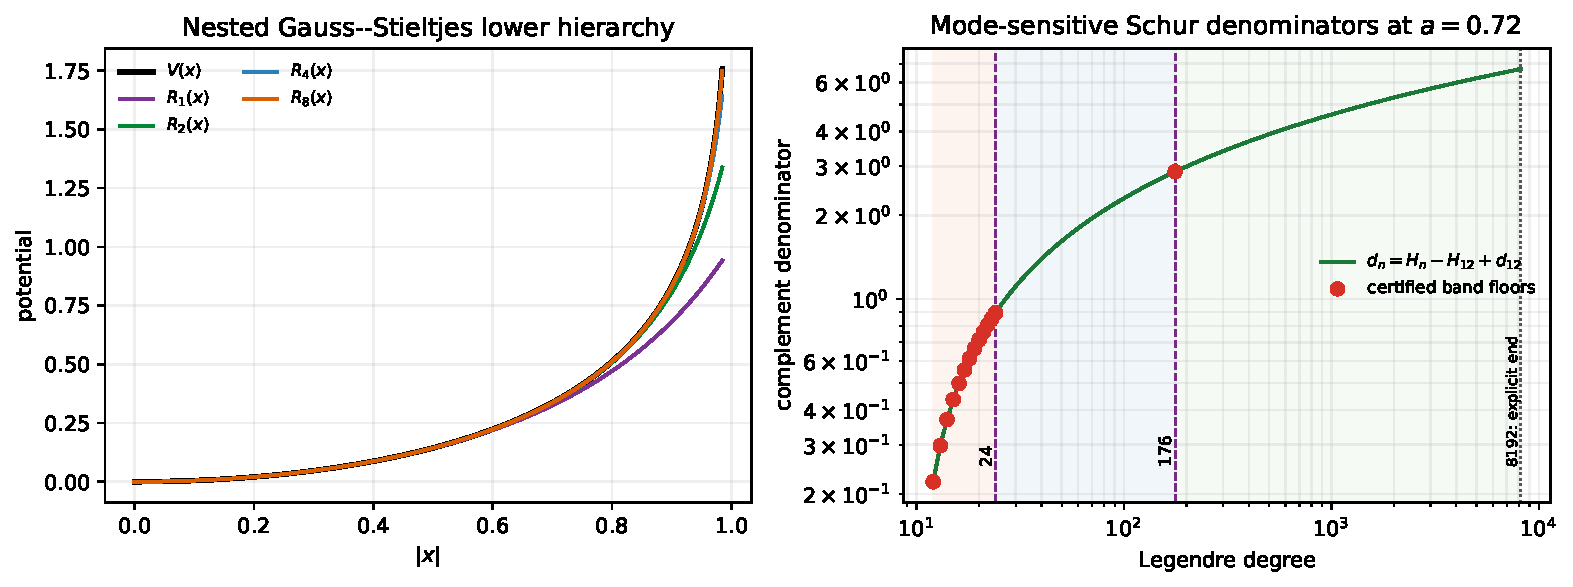
\includegraphics[width=\linewidth]{figures/stieltjes_and_multiband.pdf}
 \caption{Left: exact nested lower approximants to the logarithmic boundary
 potential.  Right: harmonic denominators and the three registered floors in
 the support-$0.72$ Schur certificate.  The plots illustrate proved formulas;
 no sampled curve decides a sign.}
 \label{fig:overview}
\end{figure}

\section{Mode-sensitive Schur complements}

We isolate the operator inequality that turns rigorous component Grams into a
full infinite-dimensional certificate.

\begin{theorem}[degree-resolved Schur majorant]\label{thm:schur}
Let $\mathcal H=\mathcal H_0\oplus\mathcal H_1$ and
\[
 T=\begin{pmatrix}A&B\\B^*&D\end{pmatrix}=T^*.
\]
Suppose $\{P_n\}_{n\ge N}$ are mutually orthogonal projections summing to the
identity on $\mathcal H_1$ and
\begin{equation}\label{eq:Dlower}
 D\succeq\sum_{n\ge N}d_nP_n,\qquad d_n>0.
\end{equation}
Then
\begin{equation}\label{eq:resolved}
 BD^{-1}B^*\preceq R_*:=
 \sum_{n\ge N}\frac{(BP_n)(BP_n)^*}{d_n}.
\end{equation}
For consecutive bands $I_j=[m_j,m_{j+1})$, define
\[
 R_{\mathcal P}=\sum_j\frac1{d_{m_j}}
 \sum_{n\in I_j}(BP_n)(BP_n)^*.
\]
If $d_n$ is increasing and $d_n\le(1+\varepsilon)d_{m_j}$ on $I_j$, then
\begin{equation}\label{eq:relative}
 R_*\preceq R_{\mathcal P}\preceq(1+\varepsilon)R_*.
\end{equation}
If $d_n=H_n+c>0$, a greedy partition through degree $M$ uses at most
\begin{equation}\label{eq:bandcount}
 1+\left\lceil\frac{\log(d_{M-1}/d_N)}
 {\log(1+\varepsilon)}\right\rceil
 =O_\varepsilon(\log\log M)
\end{equation}
bands.
\end{theorem}
\begin{proof}
Inverse antitonicity on positive operators applied to \eqref{eq:Dlower}
gives
$D^{-1}\preceq\sum d_n^{-1}P_n$, hence \eqref{eq:resolved}.
On a band,
$d_n^{-1}\le d_{m_j}^{-1}\le(1+\varepsilon)d_n^{-1}$; multiply by each
positive Gram and sum.  Greedy band starts make successive denominators grow
geometrically, and $H_M\sim\log M$ gives \eqref{eq:bandcount}.
\end{proof}

\begin{lemma}[interval congruence judge]\label{lem:congruence}
Let $S=S^*$ on $\R^r$, and let $X$ be a real square matrix.  If interval
arithmetic proves
\[
 X^TX\preceq u\Id,\qquad X^TSX\succeq g\Id,
 \qquad 0<g,\quad u<\infty,
\]
then $X$ is invertible as soon as a positive lower bound for $X^TX$ is also
certified, and
\begin{equation}\label{eq:congruence-transport}
 S\succeq \frac gu\Id.
\end{equation}
It is enough to establish both matrix inequalities by outward-rounded
Gershgorin bounds.
\end{lemma}
\begin{proof}
For $z=Xy$, one has
$y^TX^TSXy\ge g\|y\|^2$ and
$\|z\|^2=y^TX^TXy\le u\|y\|^2$.
The positive lower Gram bound makes $X$ onto, so \eqref{eq:congruence-transport}
holds for every $z$.
\end{proof}

\begin{lemma}[full block coercivity]\label{lem:block-coercivity}
For the block operator in \cref{thm:schur}, suppose
\[
 D\succeq d\Id,\qquad
 A-BD^{-1}B^*\succeq s\Id,\qquad \|B\|\le b,
 \qquad d,s>0.
\]
Then
\begin{equation}\label{eq:full-coercivity}
 T\succeq
 \left(\frac{(1+b/d)^2}{s}+\frac1d\right)^{-1}\Id.
\end{equation}
If $BB^*\preceq G$, the computable substitution
$b\le\sqrt{\Tr G}$ is valid.
\end{lemma}
\begin{proof}
Put $w=v+D^{-1}B^*u$.  Block Gaussian elimination gives
\[
 \ip{(u,v)}{T(u,v)}\ge s\|u\|^2+d\|w\|^2.
\]
Moreover
$\|(u,v)\|\le(1+b/d)\|u\|+\|w\|$.
Weighted Cauchy--Schwarz proves \eqref{eq:full-coercivity}.
The trace bound follows from $\|B\|^2=\|BB^*\|\le\Tr G$.
\end{proof}

This theorem does not require $D$ to preserve the individual degree spaces.
That point is essential: \eqref{eq:Dlower} is a form inequality, and inverse
antitonicity supplies the comparison without an invariance assumption.  The
Schur--Feshbach principle then says that positivity of
$A-R_{\mathcal P}$ suffices for positivity of $T$.  The two lemmas state
exactly how an interval sign on that finite Schur matrix is transported back
to a scalar lower bound for the full operator.

\section{The support-0.72 certificate}

\subsection{Frozen architecture}

We now list every load-bearing parameter.  The finite source uses the exact
thirteen-interval graph and twelve local Legendre modes per interval.  The
complement starts at local degree 12, the explicitly enclosed tail ends at
8192, the analytic smooth expansion has order 47, and all proof balls use
512-bit precision.  The successful partition is
\begin{equation}\label{eq:split}
 [12,13),\ldots,[23,24),\qquad[24,176),\qquad[176,\infty).
\end{equation}
The first and last finite-band denominator bounds, together with the far-tail
bound, are
\begin{equation}\label{eq:denoms}
 d_{12}\ge0.2209732158977950,\quad
 d_{24}\ge0.8937207154406235,\quad
 d_{176}\ge2.868300416471574.
\end{equation}
The twelve degreewise bounds increase monotonically between $d_{12}$ and
$d_{23}\ge0.8520540487739568$.

\begin{center}
\begin{tabular}{@{}ll@{}}
\toprule
proof item & frozen value\\
\midrule
support and active prime powers & $a=0.72$; $n=2,3,4$\\
translation components & $7+4+2=13$ intervals\\
local source degrees & $0,\ldots,11$ on every interval\\
source/parity dimensions & $156=78+78$\\
explicit complement range & $12\le n<8192$\\
smooth/self remainder endpoints & $47$ and $32768$\\
pointwise subdivisions & $1024$\\
ball precision & $512$ bits\\
\bottomrule
\end{tabular}
\end{center}

\subsection{Fail-closed finite reduction}

The aggregate $[12,176)$ coupling Gram is generated independently from twelve
nonzero degreewise Grams on $[12,24)$.  The residual $[24,176)$ Gram is formed
as an Arb interval subtraction, not by subtracting floating midpoints.
Endpoint flux, adjacent
singular, other-tail, and directional self-tail contributions enter as Grams
before the final Schur subtraction.

For each parity $\pi$, the verifier performs the following fixed sequence.
\begin{enumerate}
\item It encloses the source matrix $A_\pi$, the aggregate Gram
$G_\pi^{[12,176)}$, the independently generated degree Grams
$G_\pi^{[m,m+1)}$ for $12\le m<24$, and the far-tail Gram.
\item It forms
$G_\pi^{[24,176)}=G_\pi^{[12,176)}-\sum_{m=12}^{23}G_\pi^{[m,m+1)}$
as an Arb matrix subtraction, retaining every entry radius.
\item It subtracts the fourteen band corrections using the registered
degreewise lower endpoints and the far-tail endpoint in
\eqref{eq:denoms}, together with the endpoint, singular, smooth, and self-tail
budgets, to obtain one interval Schur matrix $S_\pi$.
\item A floating midpoint eigensystem proposes $X_\pi$.  The sign decision is
then repeated entirely in Arb: positive lower Gram for $X_\pi^TX_\pi$,
strict Gershgorin positivity for $X_\pi^TS_\pi X_\pi$, and the transport in
\cref{lem:congruence}.
\item Any nonpositive denominator, noninvertible Gram, overlapping
Gershgorin disc, metadata mismatch, or unresolved coercive lower endpoint
aborts rather than returning a sign.
\end{enumerate}

\begin{table}[H]
\centering
\caption{Final interval adjudication at $a=0.72$.}
\label{tab:certificate}
\begin{tabular}{@{}lrrrr@{}}
\toprule
sector & negative & positive & unresolved & Schur lower\\
\midrule
even & 0 & 78 & 0 & $1.550\times10^{-14}$\\
odd  & 0 & 78 & 0 & $4.368\times10^{-11}$\\
\bottomrule
\end{tabular}
\end{table}

\subsection{Return to the full Hilbert space}

For each parity, a floating midpoint eigenbasis proposes a change of basis.
The verifier then proves with Arb that its Gram is positive, so the change is
invertible, and that the congruent Schur interval is strictly Gershgorin
positive.  Finally, an interval upper bound on the squared norm of the change
of basis transports the lower bound to the original coordinates.  The block
reconstruction, including the complement and coupling norm, gives respectively
$5.890\times10^{-17}$ and
$1.652\times10^{-13}$ in the even and odd sectors.  The smaller
number proves \eqref{eq:main} by Lemma~\ref{lem:block-coercivity}; this last step
charges the norm of the source--complement coupling and is not an inference
from the finite Schur eigenvalue alone.

\begin{remark}[why a finite eigenvalue is insufficient]
Rayleigh--Ritz gives upper bounds on the lowest eigenvalue.  The proof instead
certifies a lower bound on the full complement, encloses the source-to-tail
coupling, and proves positivity of the resulting interval Schur matrices.
Every omitted infinite direction is charged before the sign is decided.
\end{remark}

\section{Reproducibility and falsification gates}

The proof source starts from
\href{https://github.com/lluiseriksson/riemann-prime-resolvent/tree/3d997887ccf4e056607c4488a708181db1d507ef}
{repository commit \texttt{3d997887ccf4e056607c4488a708181db1d507ef}};
the release includes the complete source snapshot and the audited accumulator
patches that produced format version 3.
Two interval proof objects and the final JSON record have the
registered names and SHA-256 digests
\begin{itemize}\small
\item \nolinkurl{theta-schur-a072-d12-p47-tail8192-v3.npz}:\\
\texttt{fab69bc8fa1d21ac0d3faca85d317ec5655fd991e7af29329329be4e5f8c1ebb};
\item \nolinkurl{theta-near-band-a072-d12-to24-by-degree-p512-v3.npz}:\\
\texttt{9119dbd4bad1a3c0de406445bbcb537e7c6d10fc6010f7a9d90ea79ae561751c};
\item \nolinkurl{theta-schur-a072-multiband-to24-by-degree-v3.json}:\\
\texttt{63b0dd91dab9fe7a00b734644c7a0400c2240a51cc25e6dde42751208dfc4f08}.
\end{itemize}
The first artifact is a deterministic outward upgrade of the allowlisted
pre-refactor aggregate: its intrinsic radii are rounded up, one centre ulp is
added, and the exact smooth remainder is rounded up.  An independent corrected
replay has identical component midpoints and strictly nonzero aggregate Grams.
The second artifact is the directly regenerated degreewise $[12,24)$ family;
the third is the theorem record.  Format version 3 records the corrected list accumulation and
centred-binary64 export, and rejects both earlier artifact schemas.
Metadata checks include support, degrees, partition, smooth order, and
precision.  The release wrapper additionally checks all expected keys,
$78\times78$ shapes, numeric finiteness, nonnegative radii, the JSON theorem
schema, and the three byte hashes before accepting a replay.  Format version 3
also widens every stored radius by one ulp of its binary64 centre, so the cache
encloses both the Arb ball and the centre-conversion displacement.  A mismatch
fails closed.

The proof is falsifiable at several levels: a nonpositive complement
denominator aborts; a nonpositive change-of-basis Gram aborts; any overlapping
Gershgorin ball is unresolved rather than rounded positive; any hash mismatch
rejects the frozen record; and parity reconstruction is checked independently
against the unreduced source.  The release includes the allowlisted predecessor,
the conservative upgrader, the fresh provenance replay, and their comparison
record; these are proof objects, not untracked assumptions.

The frozen environment is Python 3.12.6, python-flint 0.9.0, NumPy 2.5.1,
SciPy 1.18.0, and mpmath 1.3.0.  The heavy component generators were run on a
Colab Pro+ CPU runtime at 512-bit Arb precision; the aggregate replay took
approximately 80 minutes on that runtime.  The final verifier takes about two
seconds and the independent shadow audit about nine seconds on the stated
desktop environment.  The public source is the linked repository commit.
The exact archive accompanying this manuscript is
\nolinkurl{Certified_Localized_Weil_Positivity_Through_}\linebreak
\nolinkurl{Support_0_72_Reproducibility.zip}, with SHA-256
\begin{center}\small
\texttt{b5ace98f5ac8951c3939ee85c4c34563}\linebreak
\texttt{668861b0c23ca3751e7e4d5b17eb2645}.
\end{center}
Its README prints both replay commands; the terminal acceptance command is
\begin{center}\small
\texttt{python~repro/verify\_release.py~repro}.
\end{center}

\section{Relation to previous work and limitations}

Yoshida and Bombieri established the localized variational setting and a first
explicit support result \cite{Yoshida1992,Bombieri2000}.  Connes--Consani and
Connes--Consani--Moscovici developed operator and spectral-triple realizations
of Weil positivity \cite{ConnesConsani2023,CCM2025}.  Suzuki's screw-function
framework supplies the precise self-adjoint operator certified here
\cite{Suzuki2026}.  Kim et al. numerically instantiate that operator and show
the severe resolution problem in its lowest branch \cite{KimEtAl2026}.

Classical inputs are not novelty claims: Gaussian quadrature, Pad\'e/Markov
remainders, Jacobi resolvents, operator inverse antitonicity, Schur complements,
and monotone convergence of forms are standard
\cite{GolubWelsch1969,FawziEtAl2019,Haynsworth1968,Simon1978,Kato1995}.
The contributions are:
\begin{enumerate}
\item a source-faithful coercivity certificate for the complete operator at
support $0.72$, rather than a positive compression;
\item a mode-sensitive arithmetic Schur construction that retains the exact
prime-power graph through $n=4$ and closes both parity sectors;
\item the specialization of the exact Stieltjes hierarchy to Suzuki's boundary
potential, including a terminating strict-positivity hierarchy at fixed
support; and
\item a multiband theorem showing that harmonic inverse tails can
be controlled with doubly logarithmic storage.
\end{enumerate}

The result has sharp logical limits.  It does not prove positivity beyond
$0.72$, does not establish support-uniform constants, does not prove RH, does
not identify zeta zeros as eigenvalues of $A_a$, and does not turn numerical
agreement with known zeros into a premise.  Further isolated endpoints would
extend the unconditional interval but would not by themselves solve the
uniform-support problem.  A global advance needs a source-side stratification
whose finite Schur sign remains controlled as new prime powers enter.

\appendix
\section{Source-to-Gram specification}

This appendix makes the software boundary explicit.  It is normative for the
certificate: every term subtracted from the finite source is listed with its
mathematical sign and the routine that encloses it.

\subsection{Finite source}

Let $I_r$ be the thirteen intervals of Proposition~\ref{prop:partition} and
let $e_{rj}$ be the normalized local Legendre mode of degree $j<12$ on $I_r$.
Write $\ell_r=|I_r|$.  The scale-free diagonal-block entries used by the
generator are
\begin{equation}\label{eq:source-diagonal}
 D^{(r)}_{jk}=\begin{cases}
 H_j+1+\displaystyle\sum_{m=1}^{j}\frac{1}{m(2m-1)(2m+1)}
       -\log2-\log(\ell_r/2),&j=k,\\[3pt]
 \displaystyle\frac{\sqrt{(2j+1)(2k+1)}}{|j-k|(j+k+1)},
       &j\ne k,\ j+k\ \text{even},\\
 0,&j+k\ \text{odd}.
 \end{cases}
\end{equation}
Cross-interval entries are exact Legendre moments of the logarithmic kernel.
The smooth archimedean remainder is expanded through power $47$.  If
$\operatorname{up}_2$ denotes the two successive outward binary64 roundings
used at generation and adjudication, its charged scalar is
\begin{equation}\label{eq:rsm}
 r_{\rm sm}:=\operatorname{up}_2\!\left(
 2a\left[\frac{2}{3}\frac{(2a/3)^{48}}{1-2a/3}
 +\frac{2a^{48}/48!}{1-a^2/(49\cdot50)}\right]\right)
 =9.2437306756331\times10^{-16}.
\end{equation}
This is an unsigned Schur-norm upper bound, not a fitted error estimate.  Thus
the unreduced source has the auditable decomposition
\begin{equation}\label{eq:source-decomposition}
 A_{\rm src}=D+K_{\rm cross}+K_{\rm smooth}
 -\bigl(\log a+\log(2\pi)+\gamma\bigr)I
 -\sum_{n=2,3,4}\frac{\Lambda(n)}{\sqrt n}\,\mathcal A_n,
\end{equation}
where $\mathcal A_n$ is the identity-block adjacency matrix of the printed
$n$-edge list.  No quadrature is used in \eqref{eq:source-decomposition}.

Reflection sends $e_{rj}$ to $(-1)^j e_{12-r,j}$.  Hence the parity isometries
$U_\pm:\mathbb R^{78}\to\mathbb R^{156}$ have paired columns
\begin{equation}\label{eq:parity-map}
 2^{-1/2}\bigl(e_{rj}\pm(-1)^j e_{12-r,j}\bigr),\qquad 0\le r<6,
\end{equation}
together with the even, respectively odd, modes of the central interval.
The implementation checks $U_\pm^TU_\pm=I$, $U_+^TU_-=0$, and reconstructs
the unreduced spectrum before exporting $U_\pm^TA_{\rm src}U_\pm$.

\subsection{Complement rows and positive Grams}

For a target interval $t$ and complement degree $q\ge12$, let
$v_{tq}\in\mathbb R^{156}$ collect the coefficients of the exact second-Green
map from all source modes into that target mode.  Its self-block entry is
\begin{equation}\label{eq:self-row}
 (v_{tq})_{tj}=\mathbf1_{q+j\ \mathrm{even}}
 \frac{\sqrt{(2q+1)(2j+1)}}{(q-j)(q+j+1)},
\end{equation}
and the adjacent and separated entries are the corresponding exact
Legendre--Green integrals, with the orientation factor $(-1)^{q+j}$ when the
source lies to the left.  The finite band Gram is therefore, before parity
reduction,
\begin{equation}\label{eq:band-gram}
 G^{J}=\sum_{t=0}^{12}\sum_{q\in J}v_{tq}v_{tq}^{T}\succeq0.
\end{equation}
All cross terms between different source intervals are retained inside each
outer product.  Formula \eqref{eq:band-gram} is evaluated independently for
each singleton band $J=[q,q+1)$, $12\le q<24$.

The endpoint-flux Gram retains rows $p_t^\pm$ at every interval endpoint and
uses the exact weights
\begin{equation}\label{eq:flux-gram}
 \sum_{q=N}^{M-1}\frac{2q+1}{2q^2(q+1)^2}
 (p_t^+-(-1)^q p_t^-)(p_t^+-(-1)^q p_t^-)^T,
\end{equation}
plus the positive $M^{-2}$ remainder.  We now define the coefficient appearing
in the adjacent-singular row without reference to software.  On a source
interval of length $\ell_r$, write
\begin{align}
 f_j^{(r)}(u)&=\sqrt{\frac{2j+1}{\ell_r}}
 P_j(2u/\ell_r-1),&
 \widetilde f_j^{(r)}(u)&=f_j^{(r)}(-u),\\
 g_k^{(t)}(u)&=\sqrt{\frac{2k+1}{\ell_t}}
 P_k(1-2u/\ell_t),&0\le u\le\ell_t.
\end{align}
Set
\begin{equation}\label{eq:C-integral}
 R_j^{t\leftarrow r}(u):=-\frac12\left[
 (\ell_t-2u)(\widetilde f_j^{(r)})'(u)
 +u(\ell_t-u)(\widetilde f_j^{(r)})''(u)\right],\qquad
 C_{t\leftarrow r}^{kj}:=\int_0^{\ell_t}
 g_k^{(t)}(u)R_j^{t\leftarrow r}(u)\,du.
\end{equation}
All functions in \eqref{eq:C-integral} are polynomials, so the generator
expands them in monomials and evaluates the integral exactly as
$\sum_{p,q}g_{kp}R_{jq}\ell_t^{p+q+1}/(p+q+1)$ in Arb.  The
adjacent-singular row is then
\begin{equation}\label{eq:singular-row}
 s_{tq,j}=-\sum_{k<12}
 \frac{\sqrt{(2q+1)(2k+1)}}{q(q+1)-k(k+1)}
 \frac{C^{t\leftarrow r}_{kj}}{q(q+1)},
\end{equation}
summed over both neighbours $r=t\pm1$ before squaring.  Finally, the retained
self-regularized row is
\begin{equation}\label{eq:self-tail-row}
 r_{qj}=\mathbf1_{q-j\ \mathrm{even}}
 \frac{\sqrt{(2q+1)(2j+1)}j(j+1)}
 {[q(q+1)-j(j+1)]q(q+1)}.
\end{equation}
Analytic remainders of \eqref{eq:singular-row} and
\eqref{eq:self-tail-row} enter as positive diagonal Grams; the remaining
non-directional map is bounded by the smaller of its Arb spectral estimate and
the Schur row--column norm.

\begin{table}[H]\small
\centering
\caption{Normative source-to-Gram map.  Every listed object is checked for
shape, finiteness, nonnegative radii, and its registered metadata.}
\label{tab:source-gram-map}
\begin{tabular}{@{}>{\raggedright\arraybackslash}p{0.18\linewidth}
>{\raggedright\arraybackslash}p{0.28\linewidth}
>{\raggedright\arraybackslash}p{0.46\linewidth}@{}}
\toprule
object & mathematical content & generator / exported field\\
\midrule
finite source & \eqref{eq:source-decomposition}, then \eqref{eq:parity-map}
& \nolinkurl{arb_third_window_source.build_arb_third_window_source};
  \nolinkurl{source_even/odd_*}\\
degree band & complete rows \eqref{eq:band-gram}, including smooth map
& \nolinkurl{arb_third_window_near_tail_gram.build_arb_third_window_near_tail_gram};
  \nolinkurl{band_i_even/odd_*}\\
endpoint flux & \eqref{eq:flux-gram} and positive remainder
& \nolinkurl{arb_third_window_flux_gram.build_arb_third_window_flux_gram};
  \nolinkurl{flux_even/odd_*}\\
adjacent singular & both neighbours combined before the Gram
& \nolinkurl{arb_third_window_singular_gram.build_arb_third_window_singular_gram};
  \nolinkurl{singular_even/odd_*}\\
directional self & \eqref{eq:self-tail-row} and diagonal remainder
& \nolinkurl{arb_third_window_self_gram.build_arb_third_window_self_gram};
  \nolinkurl{self_even/odd_*}\\
other tail & adjacent/separated analytic comparison matrix
& \nolinkurl{arb_third_window_other_tail.certify_third_window_other_tail};
  \nolinkurl{other_tail_norm}\\
final sign & multiband Schur, Arb congruence--Gershgorin, Lemma~\ref{lem:block-coercivity}
& \nolinkurl{third_window_multiband_schur_certificate.certify_third_window_multiband_schur}\\
\bottomrule
\end{tabular}
\end{table}

\subsection{One-line reconstruction of the certificate}

With $\eta=0.2$, $\rho=10^{-4}$, and $\epsilon_{\rm oth}$ the certified
other-tail norm, define
\begin{align}
 G_{\rm str}&=2(G_{\rm flux}+G_{\rm sing}),\\
 G_{\rm tail}&=(1+\rho)\bigl((1+\eta)G_{\rm str}
 +(1+\eta^{-1})G_{\rm self}\bigr)
 +(1+\rho^{-1})\epsilon_{\rm oth}^2I.\label{eq:tail-majorant}
\end{align}
For each parity the exact matrix submitted to the interval sign test is
\begin{equation}\label{eq:final-schur}
 S_\pi=A_{{\rm src},\pi}-r_{\rm sm}I
 -\sum_{m=12}^{23}\frac{G_\pi^{[m,m+1)}}{d_m}
 -\frac{G_\pi^{[24,176)}}{d_{24}}
 -\frac{G_{{\rm tail},\pi}}{d_{176}}.
\end{equation}
The residual band is formed as an interval subtraction
$G^{[24,176)}=G^{[12,176)}-\sum_{m=12}^{23}G^{[m,m+1)}$.
Thus \eqref{eq:final-schur} fixes every sign, denominator, and remainder used
in Table~\ref{tab:certificate}.

For completeness, Table~\ref{tab:block-transport} prints the three outward
endpoints inserted in Lemma~\ref{lem:block-coercivity}: $s$ is the certified
Schur lower bound, $d$ the complement lower bound, and $b$ the coupling-norm
upper bound.  Substitution into \eqref{eq:full-coercivity} reproduces the last
column directly.
\begin{table}[H]\small
\centering
\caption{Full-block transport constants.}
\label{tab:block-transport}
\begin{tabular}{@{}lrrrr@{}}
\toprule
sector & $s$ (lower) & $d$ (lower) & $b$ (upper) & full lower bound\\
\midrule
even & $1.5503334138073538\,10^{-14}$ & $0.220973215897795$
& $3.364050436902478$ & $5.890068275105137\,10^{-17}$\\
odd & $4.368297840510665\,10^{-11}$ & $0.220973215897795$
& $3.3712214851682476$ & $1.6529959078469627\,10^{-13}$\\
\bottomrule
\end{tabular}
\end{table}

\section{Independent reconstruction audit}

The release contains \nolinkurl{independent_reference_audit.py}.  It imports
neither project modules nor python-flint.  From the printed cut points it
reconstructs all eleven prime-power edges, verifies the $78+78$ parity
isometries, loads only the raw component balls, and independently evaluates
\eqref{eq:tail-majorant}--\eqref{eq:final-schur} with 100-decimal mpmath
arithmetic.  Weyl's inequality is then applied using the maximum radius row
sum.  The shadow margins are
\[
 \lambda_{\min}(M_+)-\|R_+\|_\infty
 >6.3113\times10^{-14},\qquad
 \lambda_{\min}(M_-)-\|R_-\|_\infty
 >4.3738\times10^{-11}.
\]
This implementation is intentionally not invoked by the Arb proof and does
not replace its directed-rounding guarantee.  Its role is orthogonal: it makes
a wrong edge list, parity convention, residual-band sign, balance factor, or
denominator fail through a separately written assembly path.  The corrected
source replay additionally regenerates the component Grams from the explicit
formula, rather than merely rereading the registered NPZ objects.

\section*{AI assistance disclosure}
AI tools assisted with literature discovery, adversarial proof checking,
software inspection, and manuscript preparation.  The author selected the
claims, reviewed the mathematical arguments and executable evidence, and is
responsible for the final text and any remaining errors.

\begin{thebibliography}{99}\footnotesize
\setlength{\itemsep}{0pt}
\bibitem{Yoshida1992}
H.~Yoshida, \emph{On Hermitian forms attached to zeta functions}, in Zeta
Functions in Geometry, Adv. Stud. Pure Math. 21 (1992), 281--325.

\bibitem{Bombieri2000}
E.~Bombieri, \emph{Remarks on Weil's quadratic functional in the theory of
prime numbers, I}, Rend. Lincei Mat. Appl. 11 (2000), 183--233.

\bibitem{ConnesConsani2023}
A.~Connes and C.~Consani, \emph{Spectral triples and $\zeta$-cycles},
Enseign. Math. 69 (2023), 93--148.

\bibitem{CCM2025}
A.~Connes, C.~Consani and H.~Moscovici, \emph{Zeta spectral triples},
arXiv:2511.22755 (2025).

\bibitem{Suzuki2026}
M.~Suzuki, \emph{Weil's quadratic form via the screw function},
arXiv:2606.09096 (2026).

\bibitem{KimEtAl2026}
T.~Kim, Y.~Hong, M.~Kim, S.~Choi, J.~Jang, J.~Shin and M.~Kim,
\emph{A numerical realization of Suzuki's Weil-quadratic-form operator: the
Archimedean spectral law, its universality, and an operator form of Weil's
positivity criterion},
arXiv:2607.24830 (2026).

\bibitem{RosenzweigStanfill2026}
M.~R. Rosenzweig and S.~J. Stanfill, \emph{On the fundamental solutions of
two nonlocal parabolic equations related to logarithmic Laplacians},
arXiv:2606.04225 (2026).

\bibitem{GolubWelsch1969}
G.~H. Golub and J.~H. Welsch, \emph{Calculation of Gauss quadrature rules},
Math. Comp. 23 (1969), 221--230.

\bibitem{FawziEtAl2019}
H.~Fawzi, J.~Saunderson and P.~A. Parrilo, \emph{Semidefinite approximations
of the matrix logarithm}, Found. Comput. Math. 19 (2019), 259--296.

\bibitem{Haynsworth1968}
E.~V. Haynsworth, \emph{Determination of the inertia of a partitioned Hermitian
matrix}, Linear Algebra Appl. 1 (1968), 73--81.

\bibitem{Simon1978}
B.~Simon, \emph{A canonical decomposition for quadratic forms with
applications to monotone convergence theorems}, J. Funct. Anal. 28 (1978),
377--385.

\bibitem{Kato1995}
T.~Kato, \emph{Perturbation Theory for Linear Operators}, Springer, 1995.
\end{thebibliography}

\end{document}
